\documentclass[11pt]{article}

\usepackage[a4paper,margin=1in]{geometry}
\usepackage{array}
\usepackage{booktabs}
\usepackage{hyperref}
\usepackage{pgfplots}
\usepackage{url}
\usepackage[capitalise,nameinlink,noabbrev]{cleveref}

\pgfplotsset{compat=1.18}
\setlength{\emergencystretch}{3em}
\newcolumntype{L}[1]{>{\raggedright\arraybackslash}p{#1}}

\newcommand{\BaseBranch}{\texttt{codebase-\allowbreak flutter}}
\newcommand{\ComposerBranch}{\texttt{result-\allowbreak flutter-\allowbreak composer-\allowbreak 2-\allowbreak 0}}
\newcommand{\GPTBranch}{\texttt{result-\allowbreak flutter-\allowbreak gpt-\allowbreak 5-\allowbreak 5}}
\newcommand{\SonnetBranch}{\texttt{result-\allowbreak flutter-\allowbreak sonnet-\allowbreak 4-\allowbreak 6}}
\newcommand{\BaseLabel}{Base}
\newcommand{\ComposerLabel}{Composer 2.0}
\newcommand{\GPTLabel}{GPT-5.5}
\newcommand{\SonnetLabel}{Sonnet 4.6}
\newcommand{\AppPath}{\texttt{flutter\_local\_first}}
\newcommand{\DevLog}{\texttt{DEVELOPMENT\_LOG.md}}
\newcommand{\AnalyzeCmd}{\texttt{flutter analyze}}
\newcommand{\TestCmd}{\texttt{flutter test}}
\newcommand{\GateCmds}{\AnalyzeCmd{} and \TestCmd{}}
\newcommand{\VerificationDate}{May~18,~2026}
\newcommand{\RepeatedPrompts}{10}
\newcommand{\ZeroCount}{0}
\newcommand{\BaseTests}{2}
\newcommand{\ComposerTests}{5}
\newcommand{\GPTTests}{6}
\newcommand{\SonnetTests}{37}
\newcommand{\BaseTestFiles}{2}
\newcommand{\ComposerTestFiles}{2}
\newcommand{\GPTTestFiles}{3}
\newcommand{\SonnetTestFiles}{4}
\newcommand{\ComposerPrompts}{\RepeatedPrompts}
\newcommand{\GPTPrompts}{\RepeatedPrompts}
\newcommand{\SonnetPrompts}{\RepeatedPrompts}
\newcommand{\ComposerCommits}{10}
\newcommand{\GPTCommits}{10}
\newcommand{\SonnetCommits}{11}
\newcommand{\ComposerFiles}{6}
\newcommand{\GPTFiles}{10}
\newcommand{\SonnetFiles}{14}
\newcommand{\ComposerInsertions}{649}
\newcommand{\GPTInsertions}{635}
\newcommand{\SonnetInsertions}{1244}
\newcommand{\ComposerDeletions}{166}
\newcommand{\GPTDeletions}{122}
\newcommand{\SonnetDeletions}{193}
\newcommand{\ComposerNetLoc}{483}
\newcommand{\GPTNetLoc}{513}
\newcommand{\SonnetNetLoc}{1051}
\newcommand{\SonnetGroups}{8}

\title{Agent Hamster Wheel: Branch-Native Evaluation of Iterative AI Code Review for Local-First Application Engineering}
\author{Hyunsoo Lee}
\date{\today}

\begin{document}
\maketitle

\begin{abstract}
AI coding agents are increasingly used as iterative maintainers: developers ask them to review an existing system, repair defects, rerun checks, and record follow-up findings. Standard repair benchmarks usually collapse this process into a final pass/fail outcome, obscuring which engineering qualities a trajectory actually accumulates. This paper presents Agent Hamster Wheel, a branch-native case study of three model-labeled repair trajectories for the same Flutter local-first notes application. Starting from \BaseBranch{}, each result branch was produced by \RepeatedPrompts{} repeated review prompts and then audited through git metrics, reproduced \GateCmds{}, test-suite structure, branch logs, and code inspection. All final branch states pass the same quality gates, but they differ sharply: Composer 2.0 concentrates on reactive UI and stream polish, GPT-5.5 repairs FTS5 lifecycle and nullable-domain defects with compact coverage growth, and Sonnet 4.6 accumulates the broadest correctness envelope, including FTS5 apostrophe behavior, domain equality, constructor invariants, and \SonnetTests{} passing tests. The contribution is not a global model ranking; it is an artifact-centered protocol for evaluating iterative agentic maintenance as a software engineering process.
\end{abstract}

\section{Introduction}
\label{sec:introduction}

Modern code-agent evaluation often treats a model as a one-shot solver: a benchmark issue is supplied, a patch is generated, and success is scored by tests or human acceptance. SWE-bench exemplifies the value of this repair-oriented methodology for real GitHub issues~\cite{jimenez2024swebench}. Real maintenance work, however, rarely ends after one patch. Engineers ask for a second review, probe edge cases, rerun tests, inspect logs, and decide whether the next change improves the artifact or merely adds churn.

Agent Hamster Wheel studies that iterative setting in a deliberately small but technically concrete system: a Flutter notes application backed by Drift and SQLite FTS5~\cite{drift,flutter,sqlitefts5}. The application is local-first in the sense of Kleppmann et al.~\cite{kleppmann2019localfirst}: state is owned locally, reactive views derive from local persistence, and correctness depends on database behavior across opens, migrations, stream subscriptions, and full-text-search maintenance.

The research question is:

\begin{quote}
When different model-labeled agents repeatedly review and repair the same local-first application from the same base branch, what kinds of engineering quality do their branches accumulate?
\end{quote}

This paper makes four contributions. First, it defines a branch-native protocol for studying repeated agent maintenance without reducing the result to a scalar leaderboard. Second, it applies the protocol to \BaseBranch{}, \ComposerBranch{}, \GPTBranch{}, and \SonnetBranch{}. Third, it separates reproduced evidence from interpretive evidence: git-derived metrics, local quality gates, test declarations, branch logs, and reviewer inspection are reported as distinct signals. Fourth, it extracts a local-first defect taxonomy covering FTS5 repair, reactive stream ownership, nullable domain semantics, test teardown, and domain-model contracts.

\section{Related Work}
\label{sec:related-work}

Repair benchmarks have made code-agent progress measurable by grounding tasks in real repositories and executable checks. Their strength is also their limitation for the present question: final acceptance says little about how a branch arrived there, which defects were discovered late, which fixes remained untested, or whether an agent revised its own earlier work. Agent Hamster Wheel complements issue-resolution benchmarks by treating branch history and development logs as evidence rather than discarding them as process noise.

The target domain also matters. Local-first applications must preserve durable local state while exposing responsive reactive views. In this setting, defects often appear outside ordinary create-read-update-delete paths: an FTS5 external-content index can become stale after trigger drift, a migration can omit repair work for already-created databases, and a widget test can hang because a reactive database stream schedules teardown asynchronously. These properties make a local-first data layer a useful stress test for iterative maintenance.

\section{Benchmark Artifact}
\label{sec:benchmark-artifact}

The benchmark subject is \AppPath{}, a Flutter package. The implementation uses Drift as a typed persistence layer over SQLite, with native FTS5 search for note title and content. The relevant code-level components are:

\begin{itemize}
  \item \texttt{AppDatabase}, which declares Drift tables for folders, notes, and note tags, sets schema version \texttt{2}, enables foreign keys, and installs the FTS5 virtual table \texttt{fts\_notes}.
  \item \texttt{NotesLocalRepository} and \texttt{FoldersLocalRepository}, which provide asynchronous operations and stream-based list APIs for UI binding.
  \item \texttt{Note} and \texttt{Folder}, the domain models whose nullable parent fields expose the copy-semantics defects discussed in \cref{sec:defect-taxonomy}.
  \item \texttt{LocalFirstNotesApp}, the Flutter shell used by widget tests to exercise the real app boundary rather than a synthetic \texttt{MaterialApp} placeholder.
\end{itemize}

The standardized prompt asks an agent to act as a principal engineer and implement a production-ready local-first data layer for a selected stack. The repository includes prompt tooling for Flutter, React Native, and Tauri trials, but this paper studies only the Flutter trial. The tracked Flutter implementation is branch-resident: \BaseBranch{} contains the common baseline, and the result branches contain the model-labeled trajectories. The active \texttt{main} checkout is therefore not treated as the benchmark subject; reproducibility depends on checking out or creating worktrees for the experiment branches.

\section{Experimental Design}
\label{sec:experimental-design}

\subsection{Branches And Process}
\label{sec:branches}

The experiment is encoded directly in git. \BaseBranch{} is the shared baseline. \ComposerBranch{}, \GPTBranch{}, and \SonnetBranch{} are final result branches named after the agent model used in the corresponding maintenance trajectory. Each result branch records \RepeatedPrompts{} review prompts in \DevLog{}; \SonnetBranch{} has \SonnetCommits{} commits rather than \RepeatedPrompts{} because one additional commit renumbers or consolidates the log.

This evidence establishes branch protocol and artifact state, not cryptographic model provenance. Accordingly, the analysis refers to the result branches as model-labeled trajectories and avoids claims about universal model superiority.

\subsection{Measurements}
\label{sec:measurements}

The study uses four evidence channels:

\begin{enumerate}
  \item \textbf{Reproduced gates}: \AnalyzeCmd{} and \TestCmd{} were run from detached worktrees on \VerificationDate{}.
  \item \textbf{Git metrics}: commits since \BaseBranch{}, changed files, insertions, deletions, and net line change were computed from branch diffs.
  \item \textbf{Test artifacts}: test files, \texttt{test(...)} declarations, \texttt{testWidgets(...)} declarations, and \texttt{group(...)} declarations were counted from the Dart test tree on each branch.
  \item \textbf{Qualitative inspection}: final code and \DevLog{} entries were inspected for named local-first correctness dimensions.
\end{enumerate}

The first three channels are reproducible from repository commands. The fourth is an expert review judgment constrained by code and tests, and \cref{tab:quality-matrix} should be read with that evidentiary boundary in mind.

\subsection{Scoring Philosophy}
\label{sec:scoring}

The protocol intentionally rejects a single scalar leaderboard. A branch can pass all tests while retaining untested defects, and a larger diff can represent either useful coverage or unnecessary churn. The comparison therefore reports gate success, artifact growth, and defect-class coverage separately. This structure asks not only whether a branch is green, but what kind of maintenance work made it green.

\section{Results}
\label{sec:results}

\begin{table}[t]
\centering
\small
\begin{tabular}{lrrrrrr}
\toprule
Trajectory & Prompts & Commits & Files & Insertions & Deletions & Tests Passed \\
\midrule
\BaseLabel{} & \ZeroCount{} & \ZeroCount{} & -- & -- & -- & \BaseTests{} \\
\ComposerLabel{} & \ComposerPrompts{} & \ComposerCommits{} & \ComposerFiles{} & \ComposerInsertions{} & \ComposerDeletions{} & \ComposerTests{} \\
\GPTLabel{} & \GPTPrompts{} & \GPTCommits{} & \GPTFiles{} & \GPTInsertions{} & \GPTDeletions{} & \GPTTests{} \\
\SonnetLabel{} & \SonnetPrompts{} & \SonnetCommits{} & \SonnetFiles{} & \SonnetInsertions{} & \SonnetDeletions{} & \SonnetTests{} \\
\bottomrule
\end{tabular}
\caption{Branch-level outcomes relative to \BaseBranch{}. All listed final states passed \GateCmds{} when reproduced from worktrees on \VerificationDate{}.}
\label{tab:branch-results}
\end{table}

\Cref{tab:branch-results} shows that pass/fail status does not discriminate between the final branches: every final state is analyzer-clean and test-clean. The branches diverge instead in the kind and scale of accumulated maintenance. \ComposerLabel{} has the smallest file-level change set and grows the suite from \BaseTests{} to \ComposerTests{} tests. \GPTLabel{} touches more files and reaches \GPTTests{} tests while concentrating on database lifecycle repair. \SonnetLabel{} has the largest diff and expands the suite to \SonnetTests{} tests across domain, repository, FTS query, and widget boundaries.

\begin{figure}[t]
\centering
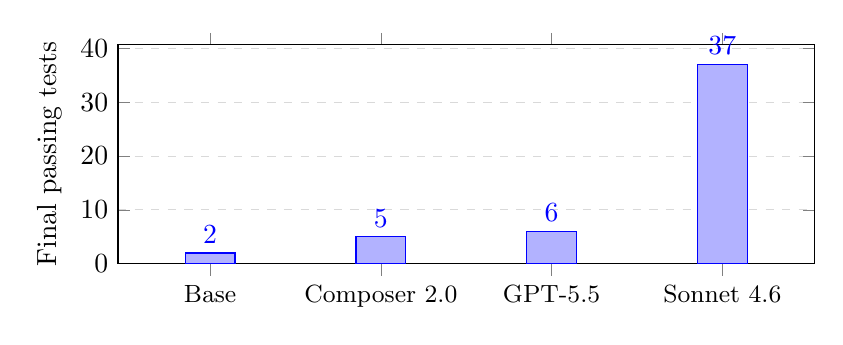
\begin{tikzpicture}
\begin{axis}[
  ybar,
  width=0.86\linewidth,
  height=0.36\linewidth,
  ymin=0,
  ylabel={Final passing tests},
  symbolic x coords={Base,C2,G55,S46},
  xtick=data,
  xticklabels={\BaseLabel{},\ComposerLabel{},\GPTLabel{},\SonnetLabel{}},
  x tick label style={font=\small},
  nodes near coords,
  nodes near coords align={vertical},
  bar width=18pt,
  enlarge x limits=0.18,
  ymajorgrids=true,
  grid style={dashed,gray!30}
]
\addplot coordinates {(Base,\BaseTests) (C2,\ComposerTests) (G55,\GPTTests) (S46,\SonnetTests)};
\end{axis}
\end{tikzpicture}
\caption{Reproduced final test counts. All branches also passed \AnalyzeCmd{}; the figure visualizes test-suite breadth rather than gate success alone.}
\label{fig:test-counts}
\end{figure}

\begin{table}[t]
\centering
\small
\begin{tabular}{lrrrr}
\toprule
Trajectory & Test Files & Test Declarations & Groups & Net LOC Change \\
\midrule
\BaseLabel{} & \BaseTestFiles{} & \BaseTests{} & \ZeroCount{} & \ZeroCount{} \\
\ComposerLabel{} & \ComposerTestFiles{} & \ComposerTests{} & \ZeroCount{} & \ComposerNetLoc{} \\
\GPTLabel{} & \GPTTestFiles{} & \GPTTests{} & \ZeroCount{} & \GPTNetLoc{} \\
\SonnetLabel{} & \SonnetTestFiles{} & \SonnetTests{} & \SonnetGroups{} & \SonnetNetLoc{} \\
\bottomrule
\end{tabular}
\caption{Test artifact growth. Net LOC is insertions minus deletions relative to \BaseBranch{}. Test declarations count \texttt{test(...)} and \texttt{testWidgets(...)} declarations.}
\label{tab:test-growth}
\end{table}

\Cref{fig:test-counts,tab:test-growth} show the main quantitative separation: \SonnetLabel{}'s larger change set is paired with a much broader explicit test oracle, whereas \ComposerLabel{} and \GPTLabel{} remain close to the baseline test scale.

\begin{table}[t]
\centering
\small
\begin{tabular}{L{0.27\linewidth}L{0.18\linewidth}L{0.18\linewidth}L{0.18\linewidth}}
\toprule
Quality Dimension & Composer 2.0 & GPT-5.5 & Sonnet 4.6 \\
\midrule
Analyzer and test gates & yes & yes & yes \\
FTS5 reopen and repair path & partial & yes & yes \\
FTS5 delete/update payload correctness & no & yes & yes \\
FTS5 apostrophe query behavior & no & no & yes \\
Nullable \texttt{copyWith} clear semantics & no & yes & yes \\
Real app widget teardown & yes & yes & yes \\
Folder empty-state or stream polish & yes & not central & partial \\
Domain equality and invariants & no & no & yes \\
\bottomrule
\end{tabular}
\caption{Qualitative quality matrix from final-branch code inspection and development logs. ``Partial'' means that a branch addresses part of the concern but leaves a relevant residual gap or treats the issue less comprehensively than another branch.}
\label{tab:quality-matrix}
\end{table}

\Cref{tab:quality-matrix} summarizes the qualitative inspection. \ComposerLabel{} primarily improves reactive UI behavior, stream binding, folder empty states, widget teardown, and FTS hydration reuse. Its residual gaps are technical rather than cosmetic: nullable \texttt{copyWith} clearing remains absent, FTS5 delete/update payloads remain under-specified, and apostrophe handling is not covered.

\GPTLabel{} concentrates on local-first persistence correctness. Its branch moves FTS5 installation into the database open path, recreates triggers, records a one-time rebuild marker, fixes update/delete payloads, repairs nullable copy semantics through sentinel values, strengthens widget teardown, and replaces default documentation with project-specific architecture notes. This trajectory addresses high-value latent defects, but it stops short of the broader domain-contract and FTS tokenization coverage present in \SonnetLabel{}.

\SonnetLabel{} accumulates the broadest engineering envelope. In addition to the FTS5 and nullable-domain fixes also present in \GPTLabel{}, it adds FTS5 apostrophe-query tests, stream churn reductions, value equality, constructor invariants, repository API symmetry, tag hydration allocation cleanup, and a later correction to keep \texttt{CREATE VIRTUAL TABLE} outside an explicit transaction. The last point is especially important for this study: a later pass identified risk in an earlier optimization and repaired the branch, demonstrating self-correction as an observable maintenance behavior.

\section{Defect Taxonomy}
\label{sec:defect-taxonomy}

The branch comparison exposes five local-first defect classes.

\paragraph{Local index correctness.}
SQLite FTS5 external-content tables depend on correct trigger payloads, trigger recreation, and index rebuild strategy. The baseline installed FTS5 infrastructure only during creation and used delete commands that did not include the old indexed title and content values. \GPTLabel{} and \SonnetLabel{} repair this class most directly.

\paragraph{Reactive stream ownership.}
Search and folder streams can churn or diverge from UI state if stream construction is tied to every rebuild or keystroke. \ComposerLabel{} improves folder stream lifecycle and UI empty states; \SonnetLabel{} also reduces search-stream churn.

\paragraph{Nullable domain semantics.}
Dart optional parameters using \texttt{??} cannot distinguish an omitted argument from an explicit \texttt{null}. \GPTLabel{} and \SonnetLabel{} introduce sentinel-based \texttt{copyWith} methods for nullable parent fields; \ComposerLabel{} leaves this baseline behavior unchanged.

\paragraph{Test-harness resource safety.}
Reactive Drift streams can leave pending timers or open database handles in widget tests if the app shell is not unmounted and drained carefully. All three result branches improve the real-app widget boundary, but the logs show different levels of teardown hardening.

\paragraph{Domain model contracts.}
As the data layer matures, domain objects need equality, hash codes, and invariants. \SonnetLabel{} is the only branch that substantially expands and tests this contract, including empty identifier checks, timestamp ordering for notes, and non-negative folder sort order.

\section{Discussion}
\label{sec:discussion}

The results support branch-native evaluation. A final gate score would label every result branch successful. The branch histories reveal a more informative profile: \ComposerLabel{} exhibits a UI/reactive maintenance bias, \GPTLabel{} prioritizes persistence lifecycle correctness, and \SonnetLabel{} pursues broader defect discovery with a much larger test oracle. These differences are not captured by \GateCmds{} alone.

The local-first domain makes those differences visible. Many important failures are history-dependent rather than simple CRUD failures: indexes go stale after an open or migration path, nullable fields fail when users clear relationships, and streams misbehave when tests or widgets tear down. Iterative maintenance evaluation should therefore include reopen paths, repair markers, stream ownership, and domain invariants alongside ordinary green tests.

\section{Threats to Validity}
\label{sec:threats}

This is a single-project case study, not a statistically powered model benchmark. The result branches are model-labeled artifacts produced under a repeated-prompt protocol; branch names and logs support the study design but do not independently authenticate model identity. The paper therefore avoids a universal ranking of Composer 2.0, GPT-5.5, and Sonnet 4.6.

The evidence sources also have different strengths. Reproduced quality gates establish final analyzer and test status on \VerificationDate{}, but they do not prove every intermediate log statement. Git metrics are exact for the repository history, while the quality matrix is an expert interpretation constrained by final code, tests, and logs. Finally, the study does not include performance microbenchmarks, blind human review, telemetry, or additional applications; those would be required before making stronger claims about runtime efficiency or general agent quality.

\section{Reproducibility}
\label{sec:reproducibility}

The branch comparison can be reproduced from the repository by inspecting branch diffs and running Flutter checks from isolated worktrees:

\begin{verbatim}
git branch --all --verbose --no-abbrev
git diff --shortstat codebase-flutter..result-flutter-composer-2-0
git diff --shortstat codebase-flutter..result-flutter-gpt-5-5
git diff --shortstat codebase-flutter..result-flutter-sonnet-4-6

git worktree add --detach /tmp/agent-hw-base codebase-flutter
git worktree add --detach /tmp/agent-hw-composer result-flutter-composer-2-0
git worktree add --detach /tmp/agent-hw-gpt result-flutter-gpt-5-5
git worktree add --detach /tmp/agent-hw-sonnet result-flutter-sonnet-4-6

cd /tmp/agent-hw-sonnet/flutter_local_first
flutter pub get
flutter analyze
flutter test
\end{verbatim}

The same Flutter commands should be run inside each worktree's \AppPath{} directory. The reproduced final counts are reported in \cref{tab:branch-results}; all listed branch states were analyzer-clean.

\section{Conclusion}
\label{sec:conclusion}

Agent Hamster Wheel demonstrates a practical evaluation pattern for iterative AI software maintenance: freeze a base branch, create one result branch per model-labeled trajectory, preserve development logs, rerun local quality gates, and compare defect classes rather than only final pass/fail status. In this repository, all three result branches pass the same Flutter gates, yet they accumulate distinct kinds of engineering quality. The central methodological lesson is that branch histories and repeated-prompt traces expose maintenance behavior that one-shot benchmark scores hide.

\bibliographystyle{plain}
\bibliography{references}

\end{document}
